\section{Groundtrack}
\label{sec:groundtrack}

The satellite's orbit is propagated to compute its groundtrack. The motion of the spacecraft is assumed to be a perturbed two body problem in Cartesian coordinates, described by the equation:

\begin{equation}
	\dot{\mathbf{r}} = -\frac{\mu}{r^3} \mathbf{r} + \mathbf{a}_{\text{perturbation}}
\end{equation}

This is solved using \textit{MATLAB}'s multi-step solver \texttt{ode113} function which is based on the Adams-Bashforth-Moulton method; it's chosen for its high accuracy over an extended period. A relative tolerance of \(1 \times 10^{-12}\) and absolute tolerance of \(1 \times 10^{-12}\) were selected for more precision.
%citation for formula: Curtis


\subsection{Unperturbed Groundtrack}

\subsubsection{Nominal Orbit Groundtrack}

The first required analysis of the ground track is for the nominal orbit considering an unperturbed case, where the $\mathbf{a}_{perturbation}$ in equation is null. The ground track was propagated for a period of 1 orbit of the satellite, 1 day and 10 days, as shown below.

\IVfig{ug1orb.eps}{ug1d.eps}{ug10d.eps}{ugstartend.png}{unpert_grountrack}{
	Ground track of the unperturbed nominal orbit during: (a) 1 orbit; (b) 1 day; (c) 10 days. Ground track path (\reddashedline), Starting point (\textcolor{red}{$\bullet$}), Ending point (\textcolor{red}{$\blacksquare$}).
}{1}

The groundtrack of this satellite has formed an “8” shape, a phenomenon known as the figure-eight groundtrack. At geosynchronous altitude, the location after one revolution is the same, and for geostationary  orbits, the satellite always appears to be stationary over one location. The figure “8” occurs because the satellites relative velocity is less and greater, than locations on the Earth as it travels from the ascending node \cite{vallado}.


\subsubsection{Repeating Groundtrack}

For establishing a good communication with the network of ground stations of PoliMi Space Agency, a repeating ground track with a ratio of 1:1 (for each orbit of the spacecraft, Earth has performed 1 revolution) is maintained. Therefore, the period of the repeating ground track orbit is computed. For an unperturbed orbit, the period is only a function of the semi-major axis and can be calculated to get the desired repeating ground track. Both equations are listed below. By extension, the other orbital parameters are kept the same as the nominal orbit. 
	
\begin{equation}
	T_{\text{repeating}} = \frac{1}{1} T_{\text{Earth}} \qquad
	T = 2\pi \sqrt{\frac{a^3}{\mu}} \rightarrow a_{\text{repeating}} = 42166 \; \text{km}
\end{equation}

\twofig{ugro1orb.eps}{ugro4orb.eps}{ground_repetition}{
	Ground track of the unperturbed repeating orbit during: (a) 1 orbit; (b) 4·k=4 orbits. Ground track path (\reddashedline), Starting point (\textcolor{red}{$\bullet$}), Ending point (\textcolor{red}{$\blacksquare$}).
}{0.85}


\subsection{Perturbed Groundtrack}

\subsubsection{Assigned Perturbations}

This project has been assigned with two perturbations: \( J_2 \) effect and Moon perturbation. \( J_2 \) effect consists of a perturbing potential on top of the central gravity field of the Earth. In order to model it, a zonal harmonic potential is used, function of the geocentric distance \( r \) and of the coelevation \( \phi \).

\begin{equation}
	R(r, \phi) = \frac{\mu}{r} \left( -1 + \sum_{n=2}^{\infty} \left( \frac{R_E}{r} \right)^n J_n P_n(\cos\phi) \right)
\end{equation}

Here, \( J_2 \) term is considered for modelling which is correlated to Earth oblateness. The perturbing acceleration due to \( J_2 \) effect is given as:

\begin{equation}
	\mathbf{a}_{J_2} = \frac{3}{2} \frac{J_2 \mu R_E^2}{r^4} \left[ \left( \frac{x}{r} \left( \frac{5z^2}{r^2} - 1 \right) \right) \mathbf{i} + \left( \frac{y}{r} \left( \frac{5z^2}{r^2} - 1 \right) \right) \mathbf{j} + \left( \frac{z}{r} \left( \frac{5z^2}{r^2} - 3 \right) \right) \mathbf{k} \right]
\end{equation}
%citation: Vallado, Curtis

Perturbation due to the moon acting on the orbit is modelled through a two body problem scenario taking into account the force of the moon as a perturbing acceleration. This acceleration is computed from:
\begin{equation}
	\label{eq:moon_perturbation}
	\mathbf{a}_{\text{Moon}} = \mu_{\text{Moon}}
	\left( \frac{\mathbf{r}_{m/s}}{r_{m/s}^3} - \frac{\mathbf{r}_m}{r_m^3} \right)
\end{equation}

where \( \mathbf{r}_{m/s} \) is the vector that goes from the S/C to the moon and \( \mathbf{r}_m \) is the vector that goes from Earth to Moon.

Possible perturbations are charted in autoref{fig:orbit perturbations}. It is observed that the \( J_2 \) effect (\( C_{2,0} \) in figure) and moon perturbation are one of the primary sources of orbital perturbation. Hence, our models and altitude choice are consistent.   

\cfig{Perturbation chart.png}{Orbit Perturbations from \cite{thesis_chart}}{orbit perturbations}{0.5}


\subsubsection{Nominal and Repeating Groundtrack}

\begin{figure}[H]
	\begin{minipage}{0.48\linewidth}
		\centering
		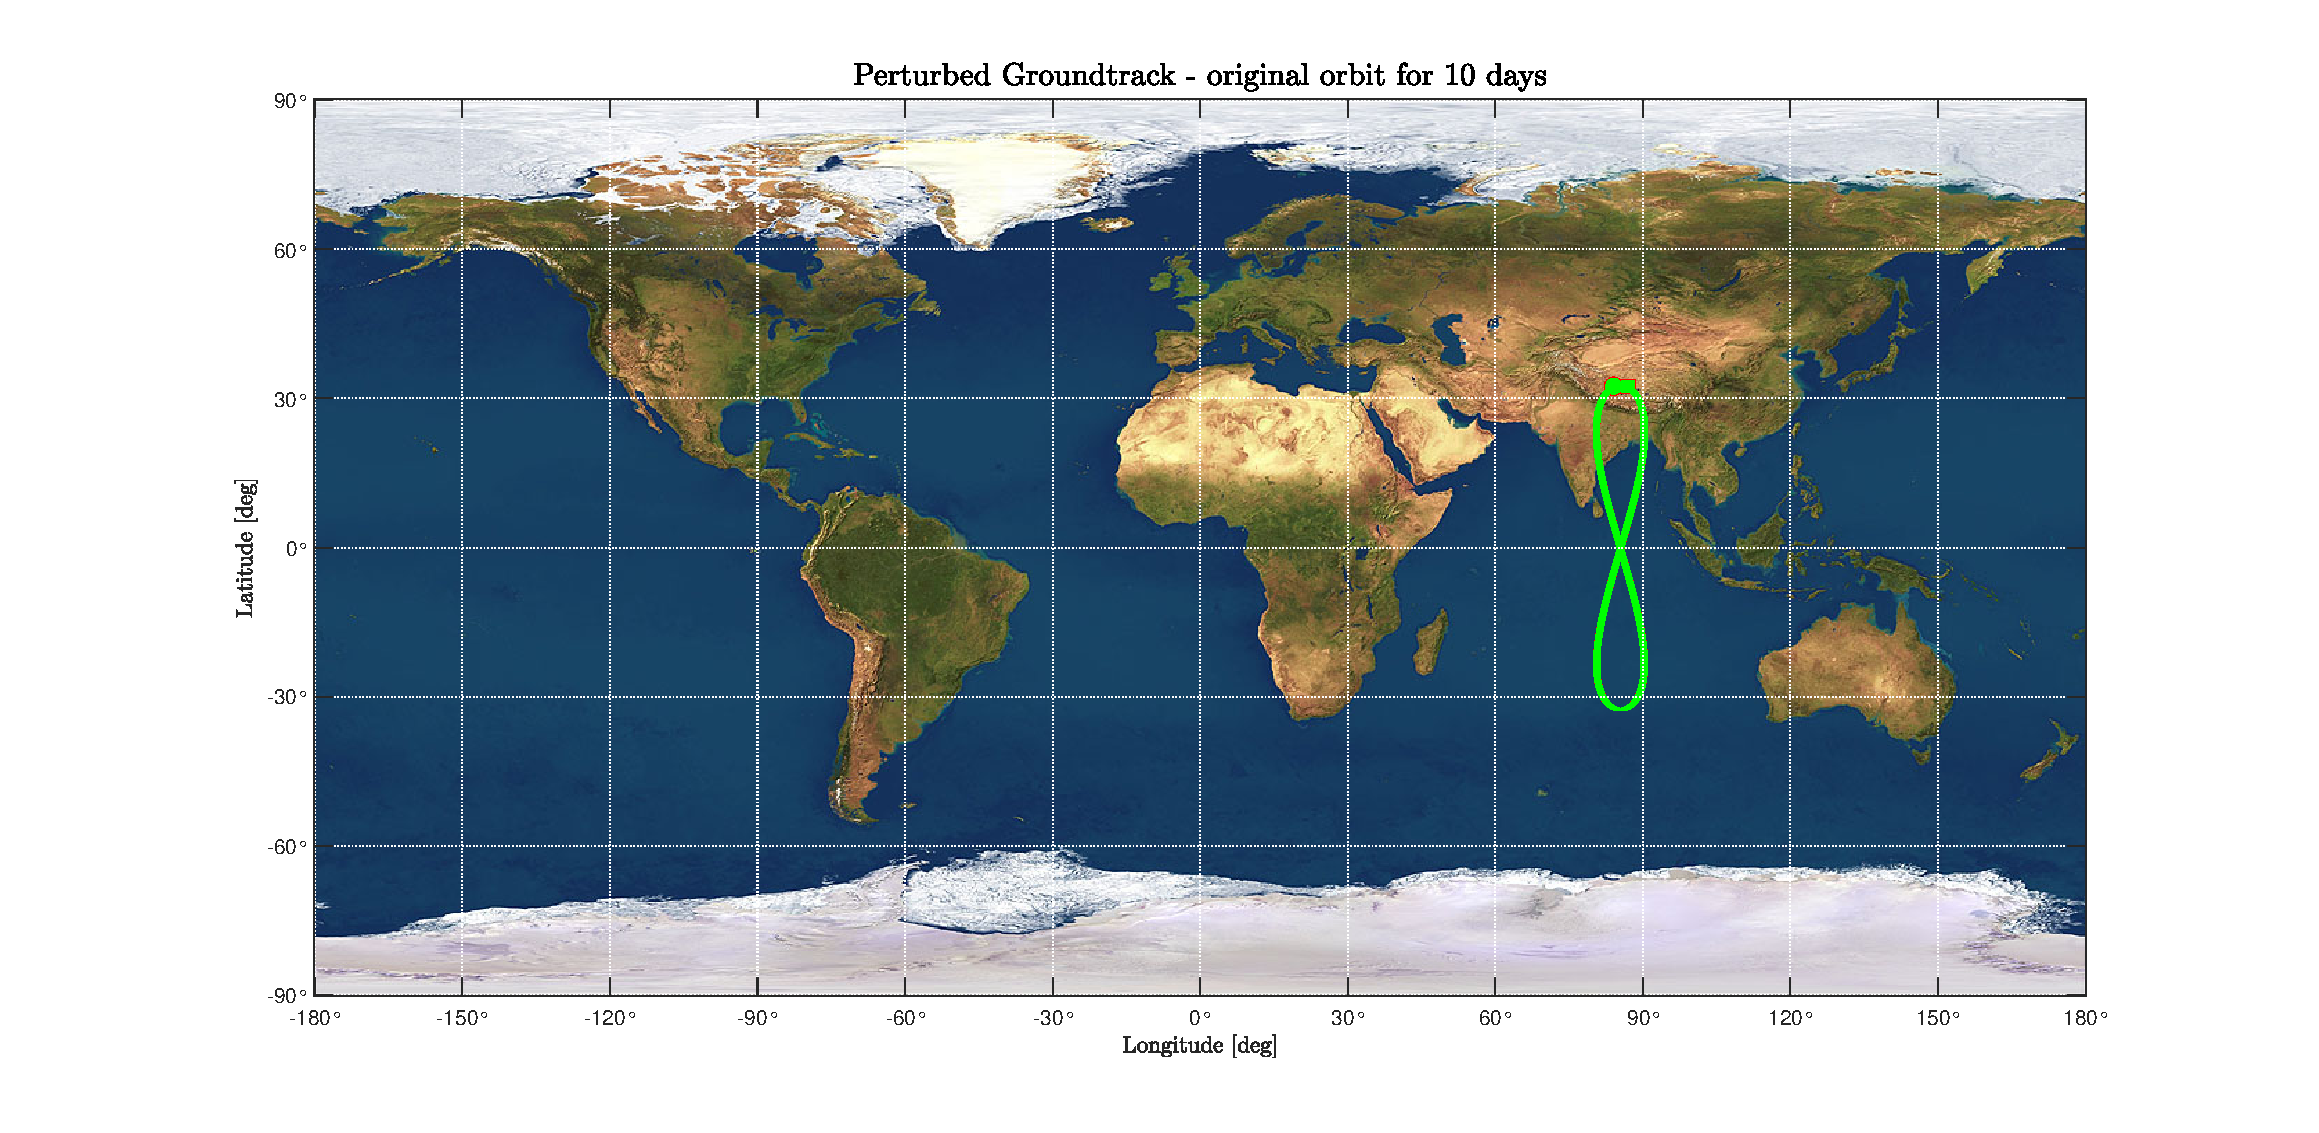
\includegraphics[width=\linewidth]{pg10d.eps}
	\end{minipage}\hfill
	\begin{minipage}{0.48\linewidth}
		\centering
		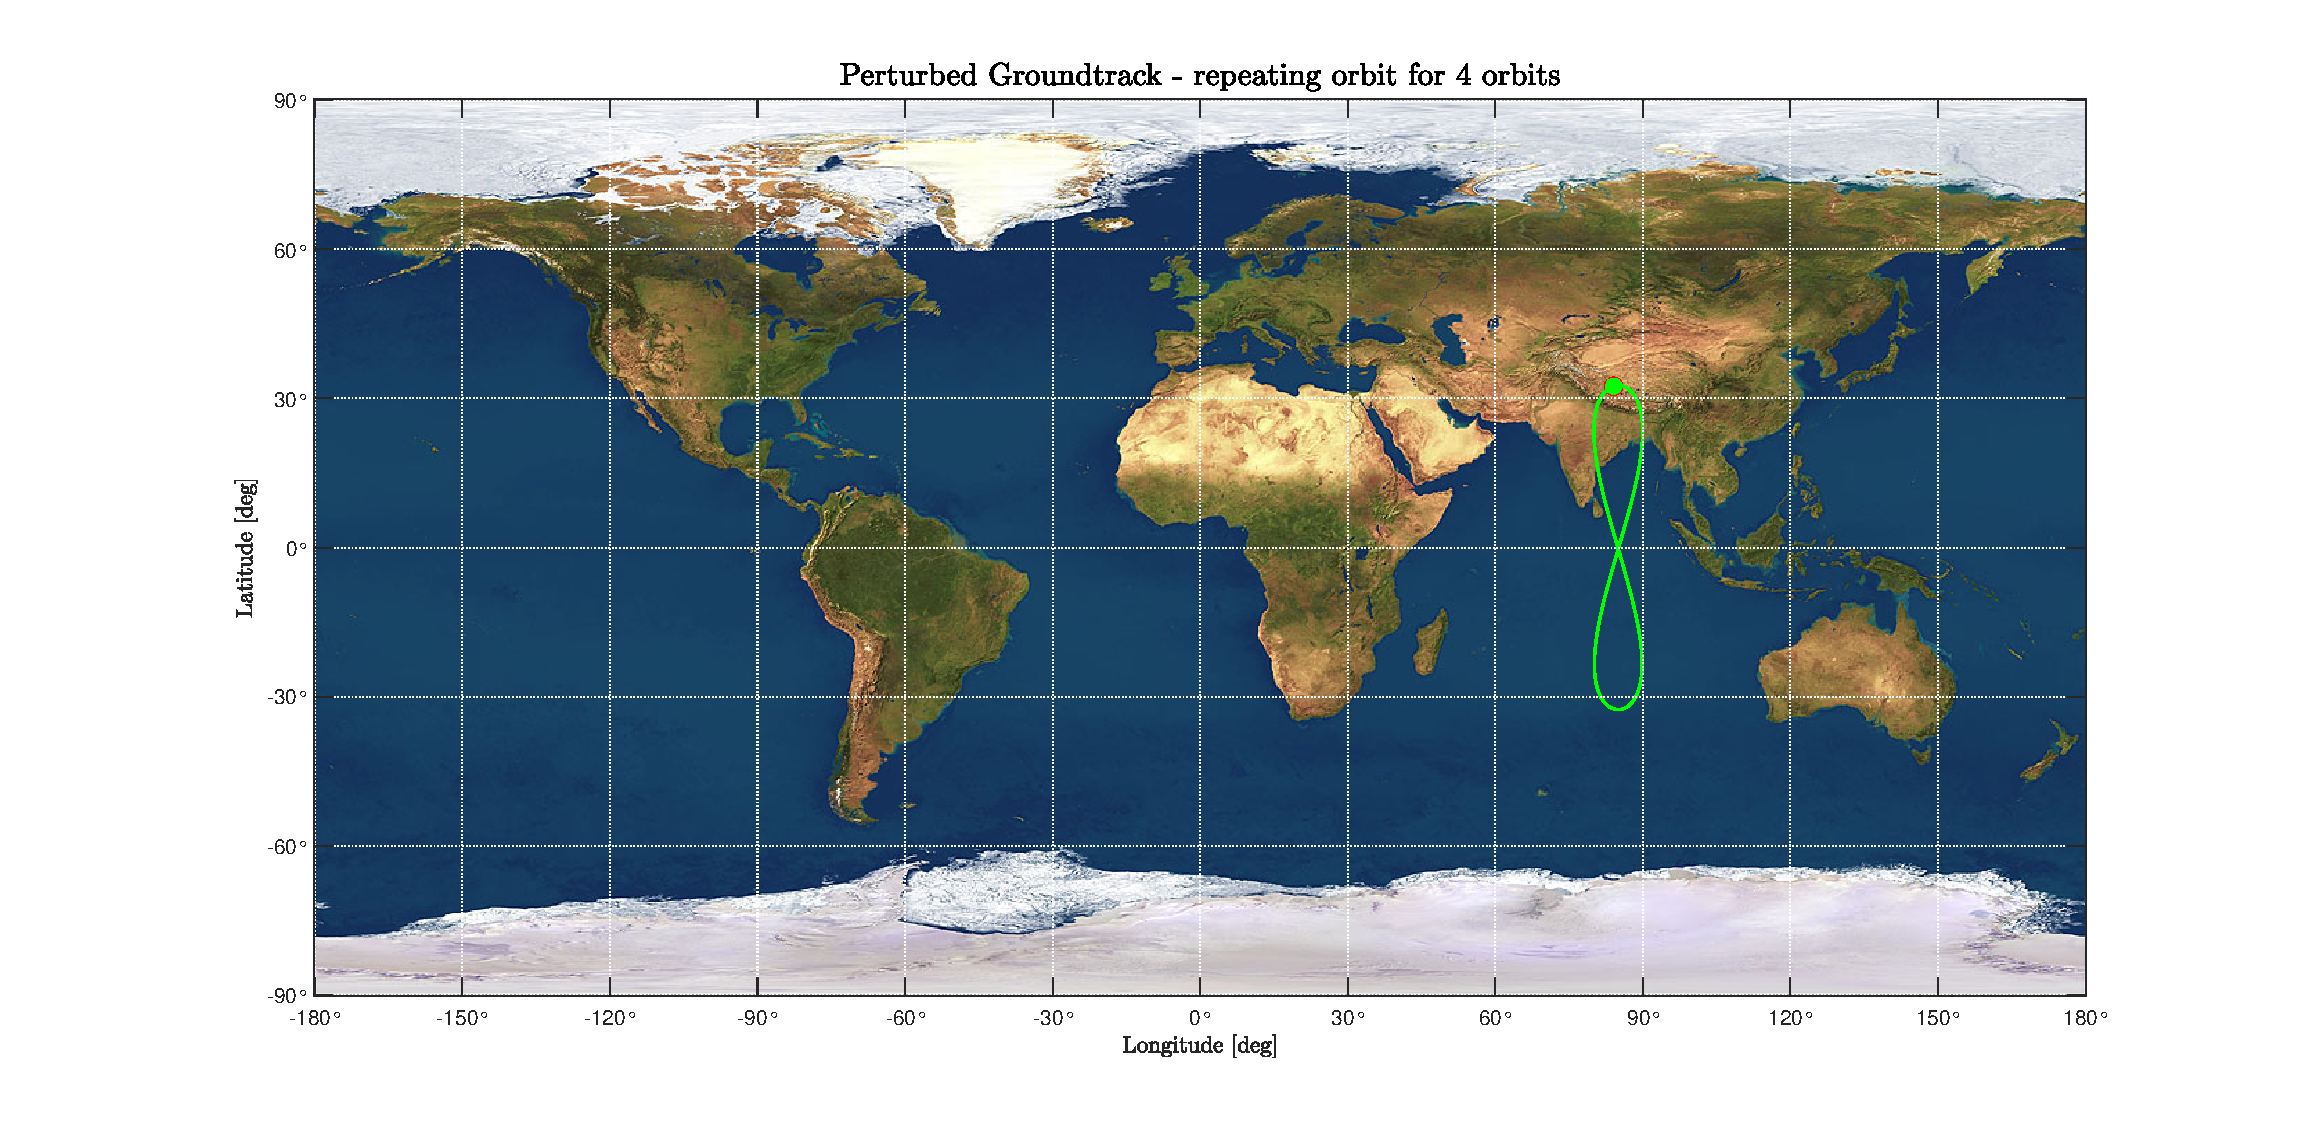
\includegraphics[width=\linewidth]{pgro4orb.eps}
	\end{minipage}
\end{figure}

\cfig{zoompgro4orb.eps}{
	Ground track of the perturbed orbits: (a) Nominal orbit during 10 days; (b) Repeating orbit during 4 orbits; (c) Perturbation effect for repeating orbit. Ground track of unperturbed (\reddashedline), Starting point (\textcolor{red}{$\bullet$}), Ending point (\textcolor{red}{$\blacksquare$}); Ground track of perturbed (\greendashedline), Starting point (\textcolor{green}{$\bullet$}), Ending point (\textcolor{green}{$\blacksquare$}).
}{groundtrack}{0.6}

It is observed that the perturbations have a great impact on the ground track path of the satellite. Both the nominal and repeating orbits get out of phase with relation to the unperturbed case. From \autoref{fig:groundtrack}, the repeating ground track orbit proposed does not work in the presence of assigned perturbations.